\documentclass[]{scrartcl}
\usepackage[most]{tcolorbox}
\usepackage{graphicx}
\usepackage{tikz}

\begin{document}

\begin{center}
	\vspace*{\fill}
	\Huge{Likelihood Free Bayesian Adaptive Estimation}
	
	\vspace{2cm}
	
	\LARGE{Jyväskylän yliopisto}\\

	\LARGE{Musiikin, taiteen ja kulttuurin tutkimuksen laitos}\\
	
	\vspace{0.25cm}
	
	\LARGE{Pro Gradu -tutkielma}\\

	\LARGE{2025}

	
	
	\vspace*{\fill}
\end{center}

\begin{minipage}{0.7\linewidth}
	\hspace{2.3in}
	\includegraphics[width=1in]{jyulogo.png}
\end{minipage}
\begin{minipage}{0.3\linewidth}
	\begin{flushright}
		Joni Pääkkö\\
		Musiikkitiede \\
		Marc Thompson
	\end{flushright}
\end{minipage}
	
\newpage

\tcbset{size=fbox,
	sharp corners,
	colframe=black,
	colback=white,
	boxrule=1.0pt,
	colbacktitle=white,
	fonttitle=\bfseries\color{black}}
\begin{tcbitemize}[
	raster equal height,raster force size=false,
	raster equal skip=0pt,raster column skip=0mm,raster columns=1]
	\tcbitem[width=1.0\linewidth]
	\textbf{Työn tekijä}\\
	Joni Pääkkö
\end{tcbitemize}

\begin{tcbitemize}[
	raster equal height,raster force size=false,
	raster equal skip=0pt,raster column skip=0mm,raster columns=1]
	\tcbitem[width=1.0\linewidth]
	\textbf{Työn otsikko}\\
	Likelihood Free Bayesian Adaptive Estimation
\end{tcbitemize}

\begin{tcbitemize}[
	raster equal height,raster force size=false,
	raster equal skip=0pt,raster column skip=0mm,raster columns=2]
	\tcbitem[width=0.5\linewidth]
	\textbf{Oppiaine}\\
	Musiikkitiede
	\tcbitem[width=0.5\linewidth]
	\textbf{Työn laji}\\
	Pro Gradu -tutkielma
\end{tcbitemize}

\begin{tcbitemize}[
	raster equal height,raster force size=true,
	raster equal skip=0pt,raster column skip=0mm,raster columns=2]
	\tcbitem[width=0.5\linewidth]
	\textbf{Aika}\\
	5.5.2025
	\tcbitem[width=0.5\linewidth]
	\textbf{Sivumäärä}\\
	85
\end{tcbitemize}

\begin{tcbitemize}[
	raster equal height,raster force size=false,
	raster equal skip=0pt,raster column skip=0mm,raster columns=1]
	\tcbitem[width=\linewidth]
	\textbf{Tiivistelmä}\\
	
	The most popular framework for formalizing adaptive testing -- at least in psychophysics -- is based on Bayesian statistics and information theory. This framework is usually employed in the context of models that, first of all, contain a likelihood function that can be evaluated in closed form and, secondly, in which responses are discrete (e.g. correct/incorrect).
	\\ \\
	This thesis generalizes the Bayesian adaptive framework to models which lack likelihood function that could be evaluated in closed form due to either its complexity or computational cost.
	\\ \\
	This more general framework can, at least in theory, be applied to a large collection of statistical models: to most, if not all, models used in psychology and related fields. This includes models in which responses are continuous, such as reaction times or ratings on a continuous scale -- these kinds of models have presented a challenge for adaptive testing in the past, despite being widely used in cognitive psychology. 
	\\ \\
	The thesis is focused on the theory of adaptive testing and does not contain any empirical research or data collection. 
	\\ \\
	The overarching structure can be divided in two parts, the first of which explicates and elaborates on the theory of adaptive testing and lays out the mathematical foundations of the titular likelihood free adaptive testing. Second part consists of numerical simulations which are used to evaluate the effectiveness of the proposed adaptive framework and to show how to practically apply it to multiple experimental paradigms that are of relevance for empirical musicological research.
	
\end{tcbitemize}

\vspace{-0.25cm}

\begin{tcolorbox}
	\textbf{Asiasanat}\\
	Adaptive testing, Bayesian statistics, Experimental Design
\end{tcolorbox}

\vspace{-0.5cm}

\begin{tcolorbox}
	\textbf{Säilytyspaikka}\\
	Jyväskylän Yliopiston kirjasto
\end{tcolorbox}


\newpage

\tableofcontents

\section{Introduction}

Arguably the most popular framework for formalizing adaptive testing is based on Bayesian statistics and information theory. 

\section{Theoretical background}

\subsection{Overview of Adaptive Testing in Psychophysics}

\subsection{Bayesian statistics}

In Bayesian statistics \textit{probability} is defined epistemologically: probability distributions are used to formalize what we \textit{know} of something. Another distinctive feature is that we begin from a formalization of \textit{prior} knowledge that is updated by making observations. 

As a simple example we know that in an unmodified deck of cards there's uniform probability for a random card to be any of the four suits. We can represent this with a uniform discrete distribution as in the left panel of Figure \ref{fig:suitsDiscUnif}

\begin{figure}[htb]
	\begin{center}
		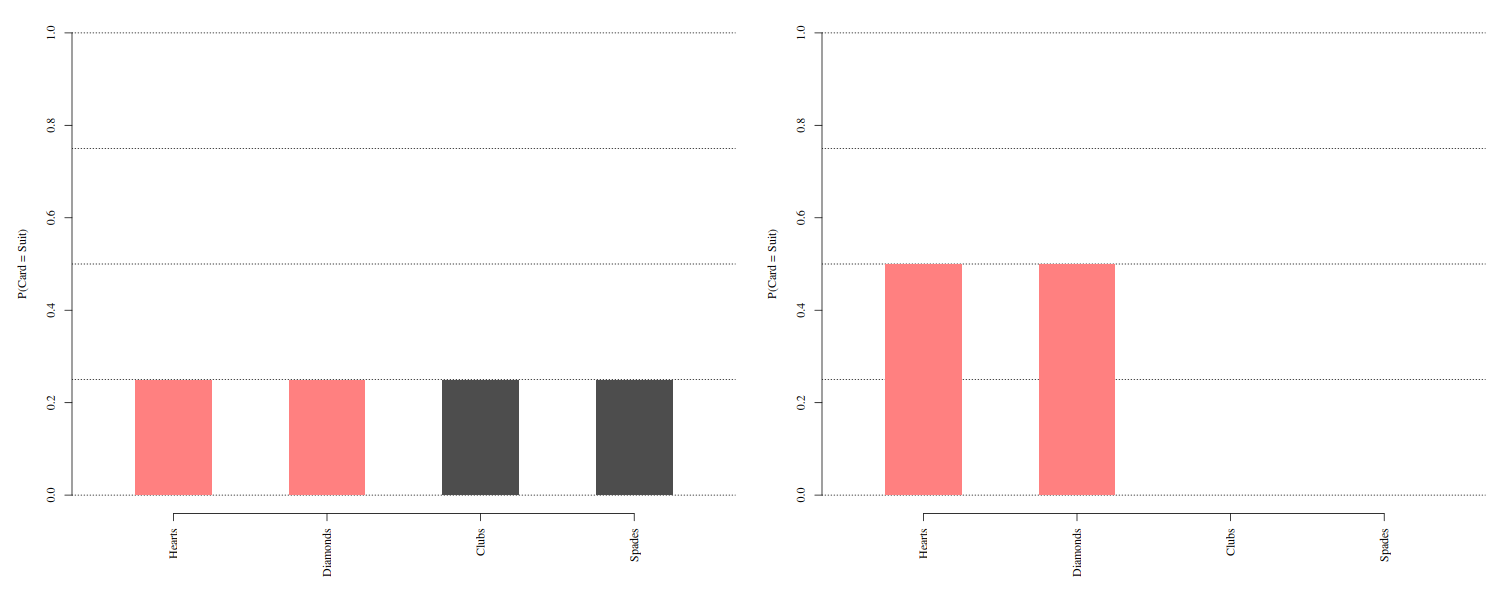
\includegraphics[width=5in]{Parts/TheoreticalBackground/Figs/discrBayes.png}
	\end{center}
	\caption{}
	\label{fig:suitsDiscUnif}
\end{figure}	

If our interrogator presents us with the knowledge that the card is red, we can update our knowledge. Now the probability of the card being clubs or spades is zero, and the probability of the card being hearts or diamonds is equal, see the right panel of Figure \ref{fig:suitsDiscUnif}. 



\begin{figure}[htb]
	\begin{center}
		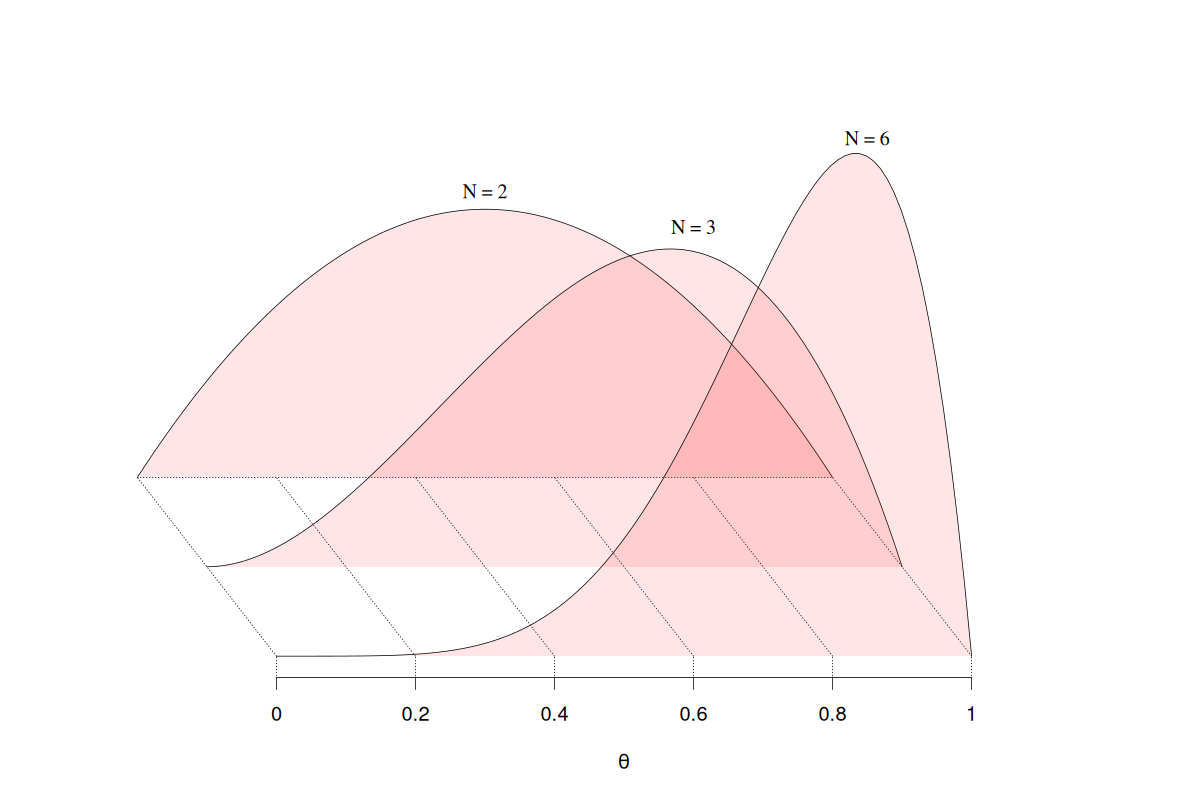
\includegraphics[width=4in]{Parts/TheoreticalBackground/Figs/sequentialBeta.png}
	\end{center}
	\caption{Demonstration of how uncertainty is reduced as more data is observed. Plausible values for the parameter $\theta$ become more and more concentrated.}
\end{figure}

\subsection{Markov Chain Monte Carlo}

\subsection{Likelihood Free Bayesian Estimation}

\subsection{Introduction to Bayesian Adaptive Testing}

\subsection{Likelihood Free Adaptive Testing}

\subsection{Entropy}

Entropy of a continuous distribution is

\begin{equation}
h[f(x)] = \int f(x)\log f(x)
\end{equation}

ERROR REFERENCE

In the continuous case we have to integrate over the 

\begin{equation}
ig(x) = h \left(\int p(y) \right)  - \int h \left( p(y) \right) 
\end{equation}

In discrete case the integrals become summations:

\begin{equation}
	ig(x) = h \left(\sum p(y) w(x)\right)  - \sum h \left(p(y)w(x)\right) 
\end{equation}

and, of course, given an IID sample, we can divide the sums with N to get the expectations:


\section{Black box algorithm}

In principle, the proposed framework could be implemented as a black box algorithm that could be used to optimize the data acquisition for any model (as defined in this thesis).

\section{Simulations}

% ERROR: Maybe this should be named something like "Applications to models"?

\subsection{Linear regression with known variance}

When variance is known, the left side reduces to a constant. This does not affect where the maximum of the information gain function is reached. This means that the left side can be dropped.

The equation

\begin{equation}
	ig(x) = h \left(\int p(y) \right)  - \int h \Bigl( p(y) \Bigl)
\end{equation}

becomes

\begin{equation}
	ig(x) = h \left(\int p(y) \right)
\end{equation}

The distribution of p(y) is a mixture of normal distributions, and consequently its entropy can not be solved in closed dorm.

\begin{figure}
	\begin{center}
		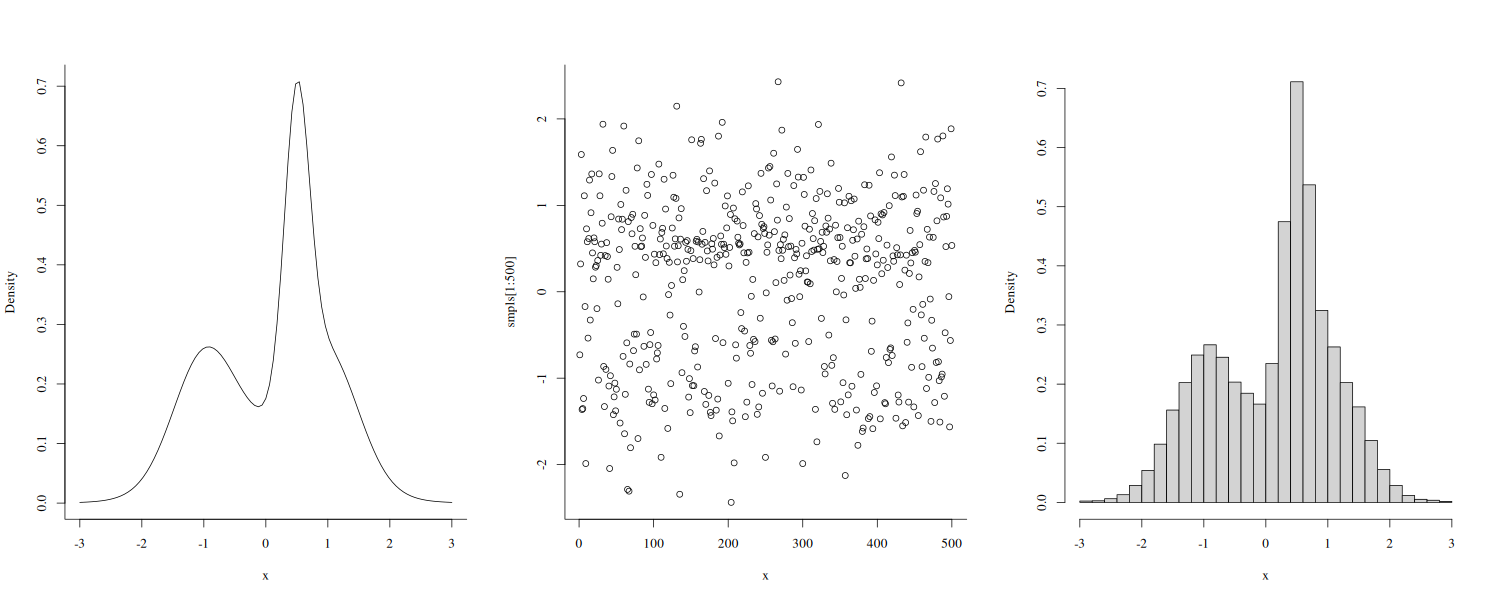
\includegraphics[width=5in]{Parts/TheoreticalBackground/Figs/etnropyApproxHist.png}
	\end{center}
	\caption{}
\end{figure}

\section{Conclusion}


\end{document}
